\documentclass[12pt]{article}
\usepackage[margin=2.5cm]{geometry}
\usepackage{enumerate}
\usepackage{amsfonts}
\usepackage{amsmath}
\usepackage{fancyhdr}
\usepackage{amsmath}
\usepackage{amssymb}
\usepackage{amsthm}
\usepackage{mdframed}
\usepackage{graphicx}
\usepackage{subcaption}
\usepackage{adjustbox}
\usepackage{listings}
\usepackage{xcolor}
\usepackage{booktabs}
\usepackage[utf]{kotex}
\usepackage{hyperref}
\usepackage{accents}

\definecolor{codegreen}{rgb}{0,0.6,0}
\definecolor{codegray}{rgb}{0.5,0.5,0.5}
\definecolor{codepurple}{rgb}{0.58,0,0.82}
\definecolor{backcolour}{rgb}{0.95,0.95,0.92}

\lstdefinestyle{mystyle}{
    backgroundcolor=\color{backcolour},
    commentstyle=\color{codegreen},
    keywordstyle=\color{magenta},
    numberstyle=\tiny\color{codegray},
    stringstyle=\color{codepurple},
    basicstyle=\ttfamily\footnotesize,
    breakatwhitespace=false,
    breaklines=true,
    captionpos=b,
    keepspaces=true,
    numbers=left,
    numbersep=5pt,
    showspaces=false,
    showstringspaces=false,
    showtabs=false,
    tabsize=1
}

\lstset{style=mystyle}

\pagestyle{fancy}
\renewcommand{\headrulewidth}{0.4pt}
\lhead{CSC 343}
\rhead{Worksheet 14 Solution}

\begin{document}
\title{CSC343 Worksheet 14 Solution}
\maketitle

\begin{enumerate}[1.]
    \item

    \bigskip

    \underline{\textbf{Notes:}}

    \bigskip

    \begin{itemize}
        \item E/R Model
        \begin{itemize}
            \item Means \textbf{Entity Relationship Model}
            \item Entity Relationship Model(ER Modeling) is a graphical approach to database design.
            \item Is comparable to class diagram in UML
            \item Uses three principle element types:

            \begin{enumerate}[1.]
                \item Entity sets
                \begin{itemize}
                    \item Is an abstract object of some sort (i.e. entitiy)
                    \item Is not used to represent class
                    \item Is represented by rectangles
                \end{itemize}

                \begin{center}
                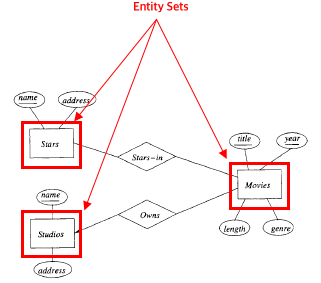
\includegraphics[width=0.7\linewidth]{images/worksheet_14_solution_1.png}
                \end{center}

                \item Attributes
                \begin{itemize}
                    \item Are properties of entities in a set (i.e. column name)
                    \item Each has its own primitive data types (e.g. String, integers, Reals)
                    \item Is represented by ovals
                \end{itemize}

                \begin{center}
                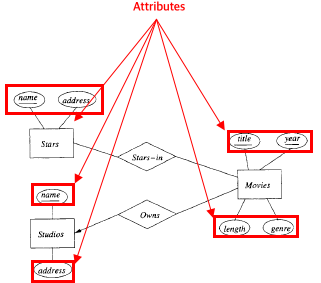
\includegraphics[width=0.7\linewidth]{images/worksheet_14_solution_2.png}
                \end{center}

                \item Relationships
                \begin{itemize}
                    \item Are connections among two or more entity sets (e.g. intermediary Relations like Stars In)
                    \item Is represented by diamond
                \end{itemize}

                \begin{center}
                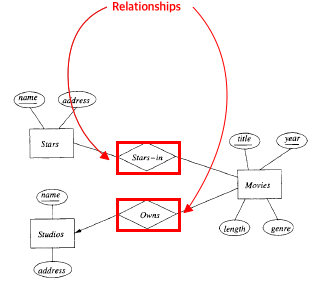
\includegraphics[width=0.7\linewidth]{images/worksheet_14_solution_3.png}
                \end{center}
            \end{enumerate}

            \bigskip

            \underline{\textbf{Example:}}

            \bigskip

            \begin{center}
            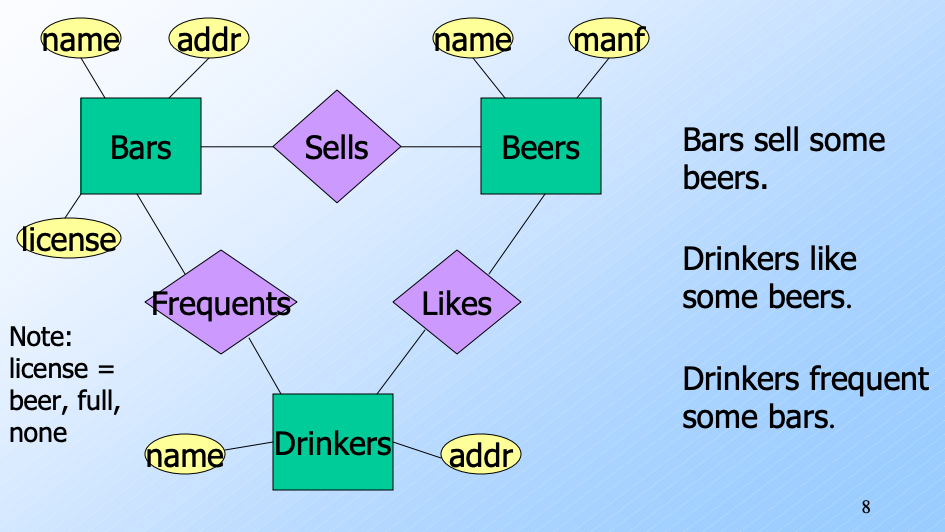
\includegraphics[width=0.7\linewidth]{images/worksheet_14_solution_4.png}
            \end{center}
        \end{itemize}
    \end{itemize}
\end{enumerate}

\end{document}